\documentclass[12pt,a4paper,openany]{book}

%Uporabljeni paketi
\usepackage[utf8]{inputenc}
\usepackage{cmap}
\usepackage{type1ec}
\usepackage[T1]{fontenc}
\usepackage{fancyhdr}
\usepackage{graphicx,epsfig}
\usepackage[slovene]{babel}
\usepackage{cite}
\usepackage{listings}
\usepackage{amsmath}

\usepackage[pdftex,colorlinks,citecolor=black,filecolor=black,linkcolor=black,urlcolor=black,pagebackref]{hyperref}
\usepackage{tikz}

\lstset{
    xleftmargin=2em,
    basicstyle= \small,
    stringstyle=\ttfamily,
    literate=%
        {č}{{\v{c}}}1
        {š}{{\v{s}}}1
        {ž}{{\v{z}}}1
        {λ}{{$\lambda$}}1
        {->}{{$\rightarrow$}}1
        {=>}{{$\Rightarrow$}}1
        {<}{{$\langle$}}1
        {>}{{$\rangle$}}1   
}

%Velikost strani - dvostransko
\oddsidemargin 1.4cm
\evensidemargin 0.35cm
\textwidth 14cm
\topmargin 0.26cm
\headheight 0.6cm
\headsep 1.5cm
\textheight 20cm

%Nastavitev glave in repa strani
\pagestyle{fancy}
\fancyhead{}
\renewcommand{\chaptermark}[1]{\markboth{\textsf{Poglavje \thechapter:\ #1}}{}}
\renewcommand{\sectionmark}[1]{\markright{\textsf{\thesection\  #1}}{}}
\fancyhead[RE]{\leftmark}
\fancyhead[LO]{\rightmark}
\fancyhead[LE,RO]{\thepage}
\fancyfoot{}
\renewcommand{\headrulewidth}{0.0pt}
\renewcommand{\footrulewidth}{0.0pt}

\newcommand{\gnuplot}{\textbf{gnuplot}}
\newcommand{\pgfname}{\textsc{pgf}}
\newcommand{\tikzname}{Ti\emph{k}Z}

%%%%%%%%%%%%%%%%%%%%%%%%%%%%%%%%%%%%%%%%%%%%%%%%%%%%%%%%%%%%%%%%
%% ccBeamer 0.1, 2007-07-02                                   %%
%% Written by Sebastian Pipping <webmaster@hartwork.org>      %%
%% ---------------------------------------------------------- %%
%% Licensed under Creative Commons Attribution-ShareAlike 3.0 %%
%% http://creativecommons.org/licenses/by-sa/3.0/             %%
%%%%%%%%%%%%%%%%%%%%%%%%%%%%%%%%%%%%%%%%%%%%%%%%%%%%%%%%%%%%%%%%


%% Images
\newcommand{\CcImageBy}[1]{%
	
\includegraphics[scale=#1]{creative_commons/cc_by_30.pdf}%
}
\newcommand{\CcImageCc}[1]{%
	
\includegraphics[scale=#1]{creative_commons/cc_cc_30.pdf}%
}
\newcommand{\CcImageDevNations}[1]{%
	
\includegraphics[scale=#1]{creative_commons/cc_dev_nations_30.pdf}%
}
\newcommand{\CcImageNc}[1]{%
	
\includegraphics[scale=#1]{creative_commons/cc_nc_30.pdf}%
}
\newcommand{\CcImageNd}[1]{%
	
\includegraphics[scale=#1]{creative_commons/cc_nd_30.pdf}%
}
\newcommand{\CcImagePd}[1]{%
	
\includegraphics[scale=#1]{creative_commons/cc_pd_30.pdf}%
}
\newcommand{\CcImageSa}[1]{%
	
\includegraphics[scale=#1]{creative_commons/cc_sa_30.pdf}%
}
\newcommand{\CcImageSampling}[1]{%
	
\includegraphics[scale=#1]{creative_commons/cc_sampling_30.pdf}%
}
\newcommand{\CcImageSamplingPlus}[1]{%
	
\includegraphics[scale=#1]{creative_commons/cc_sampling_plus_30.pdf}%
}


%% Groups
\newcommand{\CcGroupBy}[1]{% zoom
	\CcImageBy{#1}%
}
\newcommand{\CcGroupByNc}[2]{% zoom, gap
	\CcImageBy{#1}\hspace*{#2}\CcImageNc{#1}%
}
\newcommand{\CcGroupByNcNd}[2]{% zoom, gap
	\CcImageBy{#1}\hspace*{#2}\CcImageNc{#1}\hspace*{#2}\CcImageNd{#1}%
}
\newcommand{\CcGroupByNcSa}[2]{% zoom, gap
	\CcImageBy{#1}\hspace*{#2}\CcImageNc{#1}\hspace*{#2}\CcImageSa{#1}%
}
\newcommand{\CcGroupByNd}[2]{% zoom, gap
	\CcImageBy{#1}\hspace*{#2}\CcImageNd{#1}%
}
\newcommand{\CcGroupBySa}[2]{% zoom, gap
	\CcImageBy{#1}\hspace*{#2}\CcImageSa{#1}%
}
\newcommand{\CcGroupDevNations}[1]{% zoom
	\CcImageDevNations{#1}%
}
\newcommand{\CcGroupNcSampling}[2]{% zoom, gap
	\CcImageNc{#1}\hspace*{#2}\CcImageSampling{#1}%
}
\newcommand{\CcGroupPd}[1]{% zoom
	\CcImagePd{#1}%
}
\newcommand{\CcGroupSampling}[1]{% zoom
	\CcImageSampling{#1}%
}
\newcommand{\CcGroupSamplingPlus}[1]{% zoom
	\CcImageSamplingPlus{#1}%
}


%********************************************

\begin{document}

% stran 1 med uvodnimi listi
\thispagestyle{empty} 

\begin{center}
{\large 
UNIVERZA V LJUBLJANI\\
FAKULTETA ZA RAČUNALNIŠTVO IN INFORMATIKO\\
}

\vspace{3cm}
{\LARGE Luka Sabotič}\\

% todo: linebreaks
\vspace{2cm}
\textsc{\textbf{\LARGE 
Implementacija rekurzivnih\\ podatkovnih tipov v programski\\ jezik MiniHaskell
}}

\vspace{2cm}
{ DIPLOMSKO DELO}\\
{ NA INTERDISCIPLINARNEM UNIVERZITETNEM ŠTUDIJU\\
}

\vspace{2cm} 
{\Large Mentor: prof. dr. Andrej Bauer}

\vfill
{\Large Ljubljana, 2023}
\end{center}

\newpage

\ \thispagestyle{empty}

\newpage

%********************************************

% stran 2 med uvodnimi listi
\thispagestyle{empty}

\vspace*{5cm}
{\small \noindent
To diplomsko delo je ponujeno pod licenco \textit{Creative Commons Priznanje avtorstva-Deljenje pod enakimi pogoji 2.5 Slovenija}
ali (po želji) novejšo različico.
To pomeni, da se tako besedilo, slike, grafi in druge sestavine dela kot tudi rezultati diplomskega dela lahko prosto distribuirajo,
reproducirajo, uporabljajo, dajejo v najem, priobčujejo javnosti in predelujejo, pod pogojem, da se jasno in vidno navede avtorja in naslov tega
dela in da se v primeru spremembe, preoblikovanja ali uporabe tega dela v svojem delu, lahko distribuira predelava le pod
licenco, ki je enaka tej.
Podrobnosti licence so dostopne na spletni strani \url{http://creativecommons.si/} ali na Inštitutu za
intelektualno lastnino, Streliška 1, 1000 Ljubljana.

\begin{center}% 0.66 / 0.89 = 0.741573033707865
  \CcImageCc{0.741573033707865}\hspace*{1ex}\CcGroupBySa{1}{1ex}
\end{center}
}

\vspace*{1.5cm}
{\small \noindent
Izvorna koda diplomskega dela, njenih rezultatov in v ta namen razvite programske opreme je ponujena pod GNU General Public License,
različica 3 ali (po želji) novejšo različico. To pomeni, da se lahko prosto uporablja, distribuira in/ali predeluje pod njenimi pogoji.
Podrobnosti licence so dostopne na spletni strani \url{http://www.gnu.org/licenses/}.
}

\begin{center} 
\ \\ \vfill
{\em
Besedilo je oblikovano z urejevalnikom besedil \LaTeX. \\ Slike so izdelane s pomočjo jezika \pgfname/\tikzname.}
\end{center}

\newpage

\ \thispagestyle{empty}

\newpage

%********************************************

% stran 3 med uvodnimi listi
\thispagestyle{empty}

Namesto te strani {\bf vstavite} original izdane teme diplomskega dela s podpisom mentorja in dekana ter \v zigom fakultete, ki ga diplomant
dvigne v študent\-skem referatu,  preden odda izdelek v vezavo!

\newpage

%********************************************

% stran 4 med uvodnimi listi je prazna 
\ \thispagestyle{empty}

\newpage

%********************************************

% stran 5 med uvodnimi listi

\thispagestyle{empty}

\vspace{1cm}
\begin{center} 
{\Large \textbf{IZJAVA O AVTORSTVU}}
\end{center}

\begin{center} 
{\Large diplomskega dela}
\end{center}

\vspace{1cm}
Spodaj podpisani/-a \hspace{0.5cm} Luka Sabotič,

\vspace{0.5cm}
z vpisno številko \hspace{0.5cm} 63200031,

\vspace{1cm}
sem avtor/-ica diplomskega dela z naslovom:
   
\vspace{0.5cm}
Implementacija rekurzivnih podatkovnih tipov v programski jezik MiniHaskell

\vspace{1.5cm}
S svojim podpisom zagotavljam, da:
\begin{itemize}
	\item sem diplomsko delo izdelal/-a samostojno pod mentorstvom 
	
	prof. dr. Andrej Bauer
	
	\item	so elektronska oblika diplomskega dela, naslov (slov., angl.), povzetek (slov., angl.) ter ključne besede (slov., 			angl.) identični s tiskano obliko diplomskega dela
	\item soglašam z javno objavo elektronske oblike diplomskega dela v zbirki ''Dela FRI''.
\end{itemize}

\vspace{1cm}
V Ljubljani, dne xx.xx.2023 \hspace{1cm} Podpis avtorja/-ice:

\newpage 

%********************************************

% stran 6 med uvodnimi listi je prazna pri dvostranskem tiskanju
\ \thispagestyle{empty}

\newpage

%********************************************

% stran 7 med uvodnimi listi

\chapter*{Zahvala}

\thispagestyle{empty}

Na tem mestu se diplomant zahvali vsem, ki so kakorkoli pripomogli k uspešni izvedbi diplomskega dela.


\newpage

%********************************************

% stran 8 med uvodnimi listi je prazna pri dvostranskem tiskanju
\ \thispagestyle{empty}

\newpage

%********************************************

% stran 9 med uvodnimi listi
\thispagestyle{empty}

$\;$ 

\vspace{5cm}
\hfill {\Large \em Morebitno posvetilo}
\thispagestyle{empty}

\newpage

%********************************************

% stran 10 med uvodnimi listi je prazna pri dvostranskem tiskanju

\ \thispagestyle{empty}

\newpage

%********************************************

\renewcommand\thepage{} 
\tableofcontents 
\renewcommand\thepage{\arabic{page}}

\thispagestyle{empty}


%********************************************

\chapter*{Seznam uporabljenih kratic in simbolov}

\thispagestyle{empty}

Seznam uporabljenih kratic in simbolov, ki morajo biti enotni v celotnem delu, ne glede na označevanje v uporabljenih virih.

%\cleardoublepage

\clearpage{\pagestyle{empty}\cleardoublepage}

%********************************************
%zacno se glavni listi, ki so numerirani z arabskimi stevilkami

\setcounter{page}{1}
\pagenumbering{arabic}

\chapter*{Povzetek}

\addcontentsline{toc}{chapter}{Povzetek}

Povzetek naj posreduje bralcu kratko vsebino dela. Zajema naj namen dela, področje, na katerega se delo nanaša,
uporabljene metode, poglavitne rezultate dela, zaključke in priporočila. 
Povzetek naj ne obsega več kot eno stran, obi\v cajno ima le 200 do 300 besed. Napiše se povsem na koncu,
ko je že jasna vsebina vseh ostalih poglavij.

Ta dokument vsebuje navodilo za izdelavo diplomskega dela v obliki in strukturi, ki je v teh navodilih predpisan za
pisanje diplomskih nalog. Struktura dokumenta je namenjena obojestranskemu tiskanju, kjer se novo poglavje vedno za\v cne na lihi strani.
V dejanski diplomi poglavja in podpogla\-vja  obi\v cajno niso tako kratka kot v teh navodilih.

Za oblikovanje tega dokumenta je bil uporabljen sistem \LaTeX.
Ve\v c o \LaTeX-u lahko izve\v s na spletni strani \texttt{http://www.ctan.org/}.
Kandidati, ki bodo svoje diplomsko delo oblikovali s pomo\v cjo
\LaTeX-a, lahko izvorno kodo tega dokumenta neposredno uporabijo kot vzorec za pisanje svoje diplomske naloge.

\vspace{1.3cm}
\noindent
{\large \bf Ključne besede:}

\vspace{0.5cm}
\noindent
diploma, mentor, zagovor, podaljšanje, pisanje, struktura


\chapter*{Abstract}

\addcontentsline{toc}{chapter}{Abstract}

Povzetek naj bo napisan v angleškem jeziku.

\vspace{1.3cm}
\noindent
{\large \bf Key words:}

\vspace{0.5cm}
\noindent
Ključne besede v angleškem jeziku.


%********************************************

todo: 
- popravi širino kodnih blokov 

- ali naj dodam poglavje sintaksa jezika, kako se definirajo funkcije in to? 

- prevedi equi in iso recursive

- prevedi sum types

- prevod enumerations in single field variants

- bloke kode sem zaključeval z ločili, je to kul?

- prevedi interpreter




\newpage
\chapter{Rekurzivni tipi}
V programiranju se vsakodnevno srečujemo z velikim številom konceptov in idej, ki nam na različne načine omogočajo iskati rešitve. Eden najbolj osnovnih in popularnih je tudi rekurzija.
V osnovi rekurzija predstavlja eleganten način reševanja zapletenih problemov z razčlenitvijo na manjše probleme iste vrste, ki se nato lahko razčlenjujejo naprej. Ta sposobnost reševanja zapletenih izzivov 
postopoma, ni le preoblikovala načina kako se programerji lotevajo kodiranja, temveč je tudi postavila temelje za ustvarjanje razreda podatkovnih struktur, imenovanih rekurzivne podatkovne strukture.

Tako kot rekurzivna funkcija pokliče samo sebe, da reši problem v manjših korakih, rekurzivni tipi opredeljujejo strukture, ki vsebujejo podatke istega tipa in ustvarjajo strukturirane 
samo-referenčne vzorce. S tem, ko dovoljujejo da so elementi strukture sestavljeni iz primerkov iste strukture, oponašajo način, kako zaznavamo in opisujemo svet okoli nas. 
Na primer datotečni sistem, kjer lahko mape vsebujejo podmape, ki pa spet vsebujejo več map in datotek. Podobno v družinskem drevesu: posamezniki imajo otroke, ki sčasoma sami 
postanejo starši. Rekurzivne strukture omogočajo, da te kompleksne odnose opišemo na preprost in intuitiven način.

V programskih jezikih podatkovne strukture predstavimo s podatkovnimi tipi. Rekurzivni podatkovni tipi so predstavitve rekurzivnih podatkovnih struktur. Rekurzivne tipe lahko ločimo na induktivne in koinduktivne. Elementi prvih lahko nosijo le končne podatke, elementi drugih pa so lahko tudi neskončni. 
Morda najbolj osnoven primer rekurzivnega tipa je seznam. Ta je lahko prazen, ali pa vsebuje urejen par nekega elementa in drugega seznama. Elementu ponavadi rečemo glava, seznamu, 
ki glavi sledi, pa rep. Tako ima poljubno dolžino, lahko je tudi prazen. Njegovo definicijo zapišemo kot:

V prikazovanju primerov bom za prazen seznam uporabljal konstruktor \lstinline{Empty}, ki ne sprejme nobenega argumenta in predstavlja odsotnost vrednosti, pogosto označena kot \lstinline{nil}. \lstinline{Element} pa predstavlja vrednost, ki je vsebovana v seznamu. Ta je seveda odvisna od tipa seznama. Če bi na primer hoteli seznam celih števil, 
bi definicija izgledala tako:
\begin{lstlisting}
data ListInt = Empty | Cons Int ListInt
\end{lstlisting}
Primer seznama celih števil, ki vsebuje elemente 1, 2 in 3:
\begin{lstlisting}
let oneToThree = Cons 1 (Cons 2 (Cons 3 Empty))
- : val oneToThree : ListInt
\end{lstlisting}

Ta seznam si lahko predstavljamo tudi kot drevo:

\begin{center}
    \begin{tikzpicture}[
        level 1/.style={sibling distance=40mm},
        level 2/.style={sibling distance=20mm},
        node/.style={inner sep=2pt}
      ]
      \node[node] {\lstinline{Cons}}
        child {
          node[node] {1}
        }
        child {
          node[node] {\lstinline{Cons}}
          child {
            node[node] {2}
          }
          child {
            node[node] {\lstinline{Cons}}
            child {
              node[node] {3}
            }
            child {
              node[node] {\lstinline{Empty}}
            }
          }
        };
      \end{tikzpicture}
\end{center}

Različne vrednosti, ki jih lahko zavzame rekurzivni tip predstavimo s konstruktorji, ki sprejmejo neko število argumentov, ki so lahko spet konstruktorji. V drevesnem prikazu tega tipa so 
konstruktorji vozlišča, argumenti pa njihovi otroci. Konstruktorji, ki ne sprejmejo nobenih argumetnov, na primer \lstinline{Empty}, so listi drevesa. V našem primeru seznama s števili 
ena do tri, poznamo dva konstruktorja: \lstinline{Cons} in \lstinline{Empty}. Drevo ima tudi liste, ki predstavljajo števila. Torej lahko podan primer razčlenimo:
\begin{enumerate}
    \item imamo seznam, ki vsebuje število 1 in nek drug seznam ali rep. Konstruktor, ki nam omogoča to strukturo je \lstinline{Cons}, ki sprejme dva argumenta: število in seznam. To sta 
    njegova otroka. Vzamemo torej prvi del definicije: \lstinline{Cons 1 rep}.
    \item Seznam, ki je `rep' seznama s številom 1, je spet seznam, ki vsebuje število 2 in nov seznam. Spet uporabimo konstruktor \lstinline{Cons} in mu podamo argumenta 2 in nov seznam, se pravi 
    \lstinline{Cons 2 rep}.
    \item Ostane nam še število 3, ki ga kot argument ponudimo tretjemu \lstinline{Cons} konstruktorju. Potrebujemo še repni seznam: \lstinline{Cons 3 rep}.
    \item Ker smo na koncu seznama, uporabimo konstruktor \lstinline{Empty} in zaključimo strukturo.
\end{enumerate}

Seznamom podoben primer so drevesa. Ta so sestavljena iz vozlišč, vsako je lahko končno, ali pa ima potomce. Ti so spet drevesa. V svetu programiranja so seznami in 
drevesa ključne podatkovne strukture, ki jih uporabljamo na različne načine. Razvijajo se inovativne implementacije in algoritmi za delo z njimi in so nujni za razumevanje programiranja.
Seveda pa so to hkrati le osnovni primeri rekurzivnih tipov. V nadaljevanju bom predstavil nekaj bolj zanimivih primerov, ki so prav tako zelo uporabni.

\section{Koinduktivni podatkovni tipi}
Seznami in drevesa so končni rekurzivni tipi, kar je lahko zelo prikladno, ker lahko hranimo njihovo celo vsebino. Lahko pa se zgodi, da porebujemo podatkovni tip, ki nam omogoča dostop do 
neomejene količine podatkov. Tu nastopijo koinduktivni tipi. Najbolj so povezani z uporabo v komunikacijah, kjer ni potrebe da se komunikacijaski kanal kdaj zapre. Take tipe najdemo v  
postopkih, ki so lahko neskončni. 

Primer koinduktivnih tipov so lačne funkcije. To so funkcije, ki sprejmejo poljubno število argumentov in vrnejo novo funkcijo, ki je lačna novih argumentov. Za njihovo definicjo 
si pomagajmo z \(\mu\)\footnote{Intuitivno si pomen operatorja \(\mu\) lahko razlagamo, kot da \(\mu x.y\) pomeni "tisti x, za katerega velja x = y".} in \emph{fix}\footnote{Intuitivna 
interpretacija izraza \emph{fix f} je "tak x, za katerega velja x = f(x)".} operatorjema:
\begin{equation}
    \mathtt{Lacna} = \mu X. (\mathtt{Argument} \rightarrow X) \notag
\end{equation}
Na primer, lahko imamo funkcijo, ki sprejme število in vrne funkcijo, ki sprejme novo število:
\begin{lstlisting}
f = fix (λf:Int -> Lacna. λn:Int. f)
- : f : Lacna
\end{lstlisting}
Opazimo, da za vsak x:Int velja x = f(x).
Ko polkičemo f, bo ta vrnila novo funkcijo, ki bo lačna novih argumentov:
\begin{lstlisting}
l_1 = f 1;
- : l_1 : Lacna
\end{lstlisting}
Rezultatu lahko nato podamo nov argument in dobili bomo enak rezultat:
\begin{lstlisting}
l_2 = l_1 2;
- : l_2 : Lacna  
\end{lstlisting}
Tako funkcijo lahko gledamo tudi kot funkcijo, ki sprejme neomejeno količino argumentov in še vedno bo lačna novih:
\begin{lstlisting}
zelo_lacna = f 1 2 3 4 5 6 7 8 9 10;
- : zelo_lacna : Lacna
\end{lstlisting}
V resnici je \lstinline{zelo\_lacna} sestavljena iz več lačnih funkcij, ki se poračunajo sproti z vsakim argumentom. Lahko bi jo zapisali tudo kot:
\begin{lstlisting}
zelo_lacna = (((((((((f 1) 2) 3) 4) 5) 6) 7) 8) 9) 10
- : zelo_lacna : Lacna
\end{lstlisting}
Tako se 1 uporabi kot argument na funkciji f, 2 na funkciji, ki jo vrne f, ko sprejme 1 in tako naprej.

Koinduktivni tipi so torej zelo uporabni, ker nam omogočajo delo z neskončnimi podatki. Vendar pa je potrebno biti previden, ker lahko hitro pride do neskončnih zank. 
Lažje jih je obvladovati v lenih programskih jezikih, ker se njihova vsebina nikoli ne izračuna do konca, vedno samo po potrebi.

Najbolj znane lačne funkcije so tokovi. To so funkcije, ki sprejmejo prazne vrednosti (\lstinline{Unit}) in vrnejo pare elementov in novih tokov:
\begin{equation}
    \mathtt{Tok} = \mu X. (\mathtt{Unit} \rightarrow {\mathtt{Element}, X}) \notag
\end{equation}
Lažji način za razumevanje tokov je, da jih gledamo kot neskončne sezname, sestavljene iz parov elementov in novih tokov. Na primer, lahko imamo tok naravnih števil:
\begin{lstlisting}
naravna = fix (λf:Int -> Tok. λn:Int. λu:Unit. 
  {n, f (n+1)}) 0;
- : naravna : Tok
\end{lstlisting}
Za delo s tako funkcijo potrebujemo še nekaj pomožnih funkcij. Najprej funkcijo, ki vrne prvi element, ali glavo toka: (imejmo 1 za indeks prvega elementa in 2 za indeks drugega)
\begin{lstlisting}
glava = λt:Tok. (t Unit).1;
- : Tok : Tok -> Int
\end{lstlisting}
in še funkcijo, ki vrne rep toka:
\begin{lstlisting}
rep = λt:Tok. (t Unit).2;
- : rep : Tok -> Tok
\end{lstlisting}
Tako lahko dostopamo do poljubnega elementa v toku:
\begin{lstlisting}
tri = glava (rep (rep (rep naravna)));
- : 3 : Int
\end{lstlisting}

Oglejmo si še nadgradnjo tokov, enostavne procese. To so funkcije, ki sprejmejo nek element in vrnejo par elementa in novega procesa:
\begin{equation}
    \mathtt{Proces} = \mu X. (\mathtt{Element} \rightarrow {\mathtt{Element}, X}) \notag
\end{equation}
Na primer, lahko imamo proces, ki sproti vrača XOR zadnjih dveh prejetih elementov:
\begin{lstlisting}
xor = fix (λf:Bool->Proces. λb_1:Bool. λb_2:Bool. 
    let new_b = xor b_1 b_2 in
    {new_b, f new_b}) true;
- : xor : Proces
\end{lstlisting}
Podobno kot pri tokovih, za delo s procesi potrebujemo pomožne funkcije, kot je na primer funkcija, ki vrne vrnjeno vrednost procesa:
\begin{lstlisting}
vrednost = λp:Proces. (p true).1;
- : vrednost : Proces -> Bool
\end{lstlisting}


\section{Equi-recursive ali Iso-recursive?}
Ko implementiramo rekurzivne tipe, se moramo slej ko prej vprašati, kaj je razlika med tipom in čemer dobimo, ko ta tip enkrat 'odvijemo'. Na primer, kaj je razlika med tipom \lstinline{List}
in njegovim enkratnim odvojem \emph{$\langle$nil:Unit, cons:{Element, List}$\rangle$}? V literatiri pojavita dva pristopa k temu vprašanju: \emph{equi-recursive} in \emph{iso-recursive}.
\subsection{Equi-recursive}
Equi-recursive pristop pravi, da je tip \emph{\(\mu\)X.F(X)} po definiciji enak njegovemu odvoju \emph{F(\(\mu\)X.F(X))}, ker oba predstavljata enaka neskončna drevesa. Ta pristop nato od 
preverjevalnika tipov zahteva, da poskrbi, da se lahko oba zapisa uporabljata kot argumenta v funkcijah in podobno.

\subsection{Iso-recursive}
Iso-recursive način, pa ubere na prvi pogled nekoliko bolj zapleteno pot. Definira dve preslikavi, ki sta med seboj inverzni. Imenujmo ju \lstinline{fold} in \lstinline{unfold}. Preslikava 
\lstinline{unfold} vzame rekurzivni tip in ga preslika v njegov prvi odvoj, torej vzame tip \(\mu\)X.T in v telesu T zamenja vse pojavitve X z celotnim rekurzivnim tipom. Na primer, v definiciji 
seznama: 
\begin{equation}
    \mu \mathtt{List.}\langle\mathtt{nil:Unit, cons:}\{\mathtt{Element, List}\}\rangle \notag
\end{equation}
preslikamo v
\begin{equation}
    \langle\mathtt{nil:Unit, cons:}\{\mathtt{Element,} \mu \mathtt{List.}\langle\mathtt{nil:Unit, cons:}\{\mathtt{Element, List}\}\rangle\}\rangle. \notag
\end{equation}
  
\lstinline{Fold} pa stori ravno obratno, torej rekurzivni tip zavije nazaj. Definiciji teh preslikav lahko tako zapišemo kot:
\begin{gather}
    \mathtt{unfold}[\mu X.T]: \mu X.T \rightarrow [X \rightarrow \mu X.T] T \notag\\
    \mathtt{fold}[\mu X.T]: [X \rightarrow \mu X.T] T \rightarrow \mu X.T \notag
\end{gather}
Ker sta preslikavi inverzni, velja:

\begin{center}
    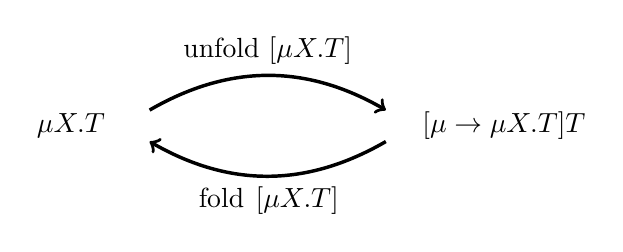
\begin{tikzpicture}
        % Left text
        \node[align=center] at (-0.5,0) {$\mu X.T$};

        % Right text
        \node[align=center] at (5,0) {$[\mu \rightarrow \mu X.T]T$};

        % Curved arrow from left to right
        \draw[->, bend left=30, line width=1.25pt] (0.5,0.2) to node[above] {\lstinline{unfold} $[\mu X.T]$} (3.5,0.2);

        % Curved arrow from right to left
        \draw[->, bend left=30, line width=1.25pt] (3.5,-0.2) to node[below] {\lstinline{fold} $[\mu X.T]$} (0.5,-0.2);
    \end{tikzpicture}
\end{center}

Tako iso-recursive pristop rekurzivni tip in njegove odvoje ne obravnava kot enake, temveč kot izomorfne.

Oba pristopa se uporabljata pri konstrukciji programskih jezikov in teoretičnih besedilih. Equi-recursive je bolj intuitiven, vednar zahteva več dela od preverjevalnika tipov in 
lahko privede do težav pri kombinaciji z drugimi konstrukti, na primer operatorjih na tipih. Medtem iso-recursive pristop zahteva uporabo preslikav \lstinline{fold} in \lstinline{unfold}, kjerkoli 
se uporabijo rekurzivni tipi. V svoji implementaciji sem uporabil iso-recursive pristop, ker je v pogosteje uporabljen, zahteva pa tudi manj dela na prevajalniku. Funkciji \lstinline{fold} in \lstinline{unfold} sta prepuščeni uporabniku.

\chapter{Vsote in variante}
Programerji se pogosto srečujemo z različnimi strukturami ali spremenljivkami, ki lahko zavzamejo vrednosti iz množice možnosti. Na primer, vozlišče v drevesu je lahko prazno, list, ali 
notranje vozlišče. Element v povezanem seznamu je lahko trivialna vrednost \lstinline{nil}, ali pa vozlišče \lstinline{Cons} z glavo in repom seznama. Takih primerov je veliko. Zato poznamo vsote.

\section{Vsote}
Vsote so tipi, ki izvirajo iz množice vrednosti, dobljene iz kombinacije natanko dveh tipov. Na primer, če imamo tipa
\begin{lstlisting}
Odrasel = {starost: Int, izobrazba: String}
Otrok = {starost: Int, šola: String}
\end{lstlisting}
za opis odraslega in otroka in želimo obravnavati oba kot en tip, da bi lahko na primer naredili seznam, ki vključuje oba tipa, lahko definiramo vsoto
\begin{lstlisting}
Oseba = Odrasel + Otrok.
\end{lstlisting}
Vsak element s tipom oseba, je tipa Odrasel, ali pa Otrok.

Za ločevanje med elementi vsote, bomo uporabljali označbe \lstinline{inl} in \lstinline{inr}. Označbi prideta iz angleških izrazov \textit{inject left} in \textit{inject right}. Lahko ju razumemo kot
funkciji, v tem primeru:
\begin{gather}
    inl: Odrasel \rightarrow Oseba \notag\\
    inr: Otrok \rightarrow Oseba \notag
\end{gather}
vendar ju bomo uporabljali zgolj kot oznaki za ločevanje med elementi vsote. Torej, elementi tipa \lstinline{Oseba} so bodisi oblike \lstinline{inl x}, kjer je x tipa \lstinline{Odrasel}, ali pa \lstinline{inr y}, kjer je y 
tipa \lstinline{Otrok}. Torej, če je \lstinline{od} tipa \lstinline{Odrasel}, je \lstinline{inl od} tipa \lstinline{Oseba}, če pa je \lstinline{ot} tipa \lstinline{Otrok}, je \lstinline{inr ot} tipa \lstinline{Oseba}.

Da lahko nato delamo z vsotami, moramo imeti funkcije, ki znajo ločevati med elementi vsote in jih obravnavati posebej. To naredimo z uporabo \lstinline{case} izraza. Če nas na primer zanimajo 
informacije o izobrazbi obravnavane osebe, lahko definiramo funkcijo izobrazba:
\begin{lstlisting}
izobrazba: λo:Oseba.
    case o of
        inl x -> x.izobrazba
        inr y -> y.šola;
\end{lstlisting}
Ko je argument o tipa Odrasel označen z \lstinline{inl}, se izvede prva veja in vrne izobrazba odraslega, ko pa je argument o tipa Otrok označen z \lstinline{inr}, se izvede druga veja in vrne šola
otroka. Tako je tip celotne funkcije \lstinline{Oseba $\rightarrow$ String}.

Preverjevalnik tipov tukaj nima težke naloge. Če imamo vsoto tipov \(T_1 + T_2\) in želimo pokazati, da je \lstinline{inl} $t_1$ tipa $T_1 + T_2$, moramo le pokazati, da je 
$t_1$ tipa $T_1$. Podobno velja za \lstinline{inr} $t_2$. Za \lstinline{case} moramo preveriti več stvari. Najprej, da je argument tipa $T_1 + T_2$. Nato preverimo 
obe veji, kjer predpostavimo da sta arumenta \lstinline{x} in \lstinline{y} tipov $T_1$ in $T_2$, v tem vrstnem redu. Preverjamo, da sta tipa $T_1$ in $T_2$ 
vrnjenih vrednosti enaka. Če je to res, označimo tip vrnjene vrednosti kot \lstinline{T}. Celoten izraz ima nato tip $T_1 + T_2 \rightarrow T$.

Ker v \lstinline{case} izrazu preverjamo tip izraza, ki je podan kot argument na način, da samo preverimo ali ustreza enemu od \(T_1\) in \(T_2\) in se ne oziramo na drugi tip v vsoti, 
se lahko zgodi, da je izrazu možno dodeliti več kot en tip. To se zgodi, če ima več vsot enak seštevanec. Za primer vzemimo vsoti \emph{$\alpha$ + $\beta$} in \emph{$\gamma$ + $\beta$}.
Obema je skupen seštevanec \emph{$\beta$}, torej lahko nekemu izrazu tipa \emph{$\beta$} dodelimo tip \emph{$\alpha$ + $\beta$} ali pa \emph{$\gamma$ + $\beta$}. To je problem, ki ga
lahko rešujemo na različne načine. V svoji implementaciji sem se odločil, da bo prevajalnik tipov izbral prvi tip, ki ga najde, torej tistega, ki je bil nazadnje definiran. To je bila 
najpreprostejša rešitev, vendar onemogoča, da bi v tem primeru tip \emph{$\beta$} kakorkoli prepoznal kot del vsote \emph{$\alpha$ + $\beta$}.

\section{Variante}
Binarne vsote lahko razširimo na variante, ki so kot vsote s poljubnim številom seštevancev. Zato označbi \lstinline{inl} in \lstinline{inr} ne prideta več v poštev, temveč uporabimo svoje oznake. 
Tako se malenkost spremeni notacija. Namesto $T_1 + T_2$ pišemo $\langle l_1:T_1, ... , l_n:T_n\rangle$, kjer \(l_i\) stoji za i-to oznako, ali label. Prav tako namesto \lstinline{inl t as} $T_1 + T_2$, pišemo $\langle l_1$ \lstinline{= t}$\rangle$ \lstinline{as} $\langle l_1:T_1, ... , l_n:T_n\rangle$. Tako naš primer z osebami postane:
\begin{lstlisting}
Oseba = <odrasel:Odrasel, otrok:Otrok>;
o = <odrasel=od> as Oseba;
- : o : Oseba

izobrazba: λo:Oseba.
    case o of
    <odrasel = od> -> od.izobrazba
      | <otrok = ot> -> ot.šola;
- : izobrazba : Oseba -> String
\end{lstlisting}


Morda zanimiva skupina variant so tiste, ki lahko vsebujejo tudi trivialne vrednosti \lstinline{unit}:
\begin{lstlisting}
Optional =  <none:unit, some:Value>;
\end{lstlisting}
Ti tipi so izomorfni s tipi, ki spadajo pod oznako \lstinline{some} in razširjeni z opcijo trivialne vrednosti. To so na primer tipi, ki jih poznamo iz priljubljenih programskih jezikov in dopuščajo 
vrednosti kot so \lstinline{null}, \lstinline{None} ali \lstinline{nil}.

Še dve posebni vrsti variant sta dovolj zanimivi za posebno obravnavo.

\subsection{Oštevilčenja (enumerations)}
Oštevilčenja so variante, ki vsebujejo zgolj trivialne vrendosti in so namenjene predstavljanju konstant. Na primer, če želimo predstaviti ocene, ki jih lahko dobi študent, definiramo varianto:
\begin{lstlisting}
Ocena = <pet:Unit, šest:Unit, sedem:Unit, osem:Unit, 
        devet:Unit, deset:Unit>;
\end{lstlisting}
Elementi takega tipa bi nato bili oblike $\langle$\lstinline{deset=unit}$\rangle$ \lstinline{as Ocena}. Tako lahko sestavimo tudi funkcije, ki obravnavajo take vrendnosti. Na primer;
\begin{lstlisting}
možno_zviševanje = λ.o:Ocena.
    case o of 
     <deset=x> -> false
    | _         -> true;
\end{lstlisting}
je funkcija, ki sprejme eno izmed ocen in vrne odgovor na vprašanje, če jo je možno izboljšati. Tip te funkcije je \lstinline{Ocena} $\rightarrow$ \lstinline{Bool}.

\subsection{Variante enega tipa (Single-field variants)}
Možno je ustvariti tudi variante s samo eno oznako, torej bodo vsi njeni elementi istega tipa:
\begin{lstlisting}
V = <l:T>;
\end{lstlisting}
torej tipa \lstinline{T}. To je lahko zelo uporabno, ker elementov tipa \lstinline{V} ni možno zamešati za elemente tipa \lstinline{T} in posledično na njih ne moremo izvajati operacij, ki jih lahko na tipu 
\lstinline{T}. Tako se lahko izognemu nesmiselnim primerom. Recimo, da uporabljamo podatke o valutah. Količino denarja v posamezni valuti lahko predstavimo s tipom \lstinline{Float}, kot decimalno 
število. Težava nastane, ko definiramo funkcijo, ki pretvarja med valutami:
\begin{lstlisting}
KuneVEvre = λx:Float. zmnoži x 0.1327;
- : KuneVEvre : Float -> Float
\end{lstlisting}
kjer \lstinline{zmnoži} predstavlja funkcijo, ki pomnoži dve decimialni števili. Če je \lstinline{x}, ki ga podamo funkciji \lstinline{KuneVEvre} količina denarja v evrih, je vse v redu. Vendar pa nam nič ne 
preprečuje, da bi kot argument v \lstinline{KuneVEvre} podali katerokoli drugo število, na primer količino denarja v dolarjih, ali še huje, število število komarjev v nekem prostoru. Taka uporaba te 
funkcije je nesmiselna in se ji v večini primerov želimo izogniti. Tako lahko definiramo variante enega tipa:
\begin{lstlisting}
DenarVKunah = <kune:Float>;
DenarVEvrih = <evri:Float>;
\end{lstlisting}
in morda še vse ostali, ki jih potrebujemo, ter funkcijo \lstinline{KuneVEvre} spremenimo tako, da deluje s pravilnimi tipi, torej pretvorbo omogočimo 
samo iz kun v evre in nič drugega:
\begin{lstlisting}
KuneVEvre = λx:DenarVKunah.
    case x of 
    <kune:x> -> <evri = zmnoži x 0.1327> 
                    as DenarVEvrih;
- : KuneVEvre : DenarVKunah -> DenarVEvrih.
\end{lstlisting}
Tako se zavarujemo pred napakami.
\newpage

\chapter{Implementacija}
Predstavljene konstrukte sem tudi sam implementiral. To sem storil v programskem jeziku MiniHaskell, ki ga je ustvaril prof. dr. Andrej Bauer in 
je dostopen na njegovem Github profilu, v repozitoriju \emph{plzoo}. 

MiniHaskell je programski jezik, ki je namenjen predstavitvi osnovnih konceptov funkcijskega programiranja. Napisan je v programskem jeziku 
OCaml in po strukturi in načinu uporabe sledi jeziku Haskell. Omogoča uporabo celih števil (\textit{integers}), booleanov z logičnimi operacijami in primerjavami 
celih števil $(`=$'$, `<$'$)$, urejenih parov, seznamov, funkcij in rekurzije. Temu sem dodal možnost definiranja novih tipov, rekurzivnih ali ne, in 
uporabe \lstinline{case} izrazov za delo z njimi. Programski jezik sestavljajo leksična analiza, razčlenjevanje, interpreter in preverjevalnik tipov. V nadaljevanju bom predstavil kako 
delujejo v MiniHaskellu, ter kako sem jih dopolnil.

\section{Leksična analiza}
Prvi korak, ki ga je potrebno narediti, ko dobimo program ali ukaz in ga želimo izvesti, je leksična analiza. To je postopek, kjer vhodni niz znakov očistimo znakov, ki ne nosijo pomembnih informacij, kot 
na primer presledki, in jih razdelimo na gradnike. To so vse ključne besede, ki jih jezik pozna, števila, znaki, \emph{eof} in podobno. To stori leksični analizator ali lekser. 
Ta je v našem primeru napisan v datoteki \emph{lexer.mll}. Je datoteka, kjer so shranjeni regularni izrazi, ki opisujejo gradnike, ki jih lahko uporabljamo v programskem jeziku. 
Kot je to storjeno v Haskellu, sem določil, da bom imena spremenljvk dovolil le z majhno začetnico, imena konstruktorjev tipov pa le z veliko. Tako sem si olajšal delo v parserju. 
Gradnik, ki bo predstavljal imena konstruktorjev in imena tipov sem poimenoval \lstinline{cname}, kot okrajšavo za \textit{capital name} ali ime z veliko začetnico. Poleg načina poimenovanja 
konstruktov je v lekserju definiranih še veliko drugih gradnikov, kot so olkepaji, znaki za operacije, ključne besede, ukaz \lstinline{:quit} za izhod iz \emph{minihaskell.exe} 
in podobno. Za definicijo podatkovnih tipov sem dodal ključno besedo \lstinline{data}, z idejo, da bo imela enako vlogo kot tista v Haskellu. Tako imamo vse potrebno za 
definicijo novih podatkovnih tipov, ker smo definirali besedo \lstinline{data}, imamo \lstinline{cname} za definicijo konstruktorjev in že od prej možnost definiranja spremenljivk.
Za delo s podatkovnimi tipi, torej izraz \lstinline{case}, je bilo potrebno dodati še gradnike za ključne besede \lstinline{case}, \lstinline{of} in \lstinline{end}.\footnote{Gradnik \lstinline{ALTERNATIVE} 
za znak '|' je že bil definiran, ker je MiniHaskell že imel sezname in funkcijo \lstinline{match} za delo z njimi.}\footnote{Gradnik \emph{TARROW} za znak \emph{$\rightarrow$}, ki bo v veji \emph{case} 
izraza ločil med izrazom, ki ga primerjamo in posledico, ki se sproži v primeru ujemanja, je prav tako že bil definiran.} V Haskellu sicer gradnika za \lstinline{end} ne poznamo, vendar ker za 
razliko od Haskella MiniHaskell ni občutljiv na zamik vrstic v kodi, in ker nisem želel z implementacijo še tega zaiti s smeri moje diplomske naloge, sem za lažje delo v parserju 
dodal tudi ta gradnik. Da bi razumeli zakaj je potreben, si poglejmo naslednji primer: recimo, da imamo \lstinline{case} izraz, ki v eni od svojih vej vsebuje še en, gnezden \lstinline{case} 
izraz:
\begin{lstlisting}
case x of 
    a -> _
    b -> case y of
            c -> _
            d -> _
    e -> _
\end{lstlisting}
Če bi bil MiniHaskell občutljiv na zamik vrstic, bi bil zgornji izraz samoumeven. Ker pa v MiniHaskellu v resnici izgleda takole:
\begin{lstlisting}
case x of a -> _ | b -> case y of c -> _ | d -> _ | e -> _,
\end{lstlisting}
ga lahko razumemo na dva načina:
\begin{lstlisting}
case x of 
    a -> _
    b -> case y of
            c -> _
            d -> _
    e -> _,
\end{lstlisting}
ali pa:
\begin{lstlisting}
case x of 
    a -> _
    b -> case y of
            c -> _
    d -> _
    e -> _.
\end{lstlisting}
Ker imajo različni programerji različna mnenja o tem, kateri od obeh je bolj smiselen in sem se želel izogniti kakeršnikoli dvoumnosti, sem dodal 
\lstinline{end} gradnik, ki nam omogoča, da enostavno določimo, kdaj se \lstinline{case} izraz konča:
\begin{lstlisting}
case x of 
    a -> _
    b -> case y of
            c -> _
            d -> _
            end
    e -> _
end.
\end{lstlisting}
Prav tako imamo v MiniHaskellu težavo z vpisovanjem izrazov na zgornji način, saj je prilagojen le vpisovanju ukazov v ukazno vsrtico, ki pa 
sprejema le nize znakov brez znaka za novo vrstico (\emph{newline} ali \lstinline{\textbackslash n}). Tako nastane težava pri iskanju meje med posameznimi vejami
\lstinline{case}-a. Haskell za to uporablja le znake za novo vrstico, jaz pa sem dodal obvezno uporabo znaka | na začetku vsake veje, ki ni prva.
Tako bi zgornji primer izgledal takole:
\begin{lstlisting}
case x of 
  a -> _
  | b -> case y of
      c -> _
      | d -> _
      end
  | e -> _
end,
\end{lstlisting}

\section{Razčlenjevanje}
Razčlenjevalnik ali parser je naslednji korak v procesu prevajanja progamov. Kot je to početo v praksi, tudi v MiniHaskellu ni parser napisan na roke, temveč 
je uporabljen program parser generator, kateremu moramo podati le slovnična pravila. Ker se tukaj uporabi Menhirjev OCaml parser generator, končnica 
datoteke ni .ml, ampak .mly. Lekser posreduje tok gradnikov, ki jih je prepoznal, naloga parserja pa je prepoznati slovnično pravilne stavke in zgraditi 
abstraktna sintaktična drevesa. To stori s pomočjo slovničnih pravil, ki povejo, v kakšnem zaporedju pričakujemo gradnike in kje se ti smejo pojaviti. 
V svoji implementaciji sem dodal dve gramatični pravili: eno za definicijo novih tipov in eno za \lstinline{case} izraz. Pravilo za definicijo novih tipov je 
sledeče:
\begin{lstlisting}
datadef:
| DATA CNAME EQUAL data_variants,

data_variants:
| data_variant
| data_variant ALTERNATIVE data_variants

data_variant:
| CNAME list(ty)
\end{lstlisting}
ki omogoča definicijo tipov na način:
\begin{lstlisting}
data Type = Constr_1 args_1 | Constr_2 args_2 | 
    ... | Constr_n args_n.
\end{lstlisting}
Seveda morajo biti TYPE in CONSTR imena z veliko začetnico. Slovnična pravila lahko zapišemo tudi z abstraktnimi sintaktičnimi drevesi. Na primer, 
definicijo tipa:
\begin{lstlisting}
data Type = Constr_1 args_1 | Constr_2 args_2 | 
    Constr_3 args_3,
\end{lstlisting}
lahko predstavimo z drevesom:
\begin{center}
    \begin{tikzpicture}[
        level 1/.style={sibling distance=60mm},
        level 2/.style={sibling distance=70mm},
        level 3/.style={sibling distance=50mm},
        level 4/.style={sibling distance=30mm},
        level 5/.style={sibling distance=10mm},
        node/.style={inner sep=2pt}
      ]
      \node[node] {\lstinline{EQUAL}}
        child {
          node[node] {\lstinline{DATA}}
			child {	
				node[node] {\lstinline{CNAME}}
			}
        }
        child {
          node[node] {\lstinline{ALTERNATIVE}}
          	child {
            	node[node] {\lstinline{CNAME}}
					child {
			  			node[node] {\lstinline{list(ty)}}
					}
          	}
          	child {
            	node[node] {\lstinline{ALTERNATIVE}}
            		child {
              			node[node] {\lstinline{CNAME}}
			  				child {
								node[node] {\lstinline{list(ty)}}
							}
					}
            		child {
              			node[node] {\lstinline{CNAME}}
			  				child {
								node[node] {\lstinline{list(ty)}}
							}
            		}
          	}
		};
      \end{tikzpicture}
\end{center}

Definicijo tipov sem kot \lstinline{datadeftop} definiral kot enega izmed štirih osnovnih ukazov. Pred njim so bili že definirani \lstinline{lettop}, ki omogoča definicijo 
spremenljivk, \lstinline{exprtop}, ki omogoča definicijo izrazov in \lstinline{cmdtop}, ki vsebuje posebne ukaze, kot so na primer \lstinline{quit}.

Slovnično pravilo za \lstinline{case} izraz pa sem dodal samo pod pravilo za \lstinline{expr} ali izraze, ker se \lstinline{case} ne uporabljav v definicijo spremenljivk ali
definiciji tipov, niti to ni poseben ukaz. Pravilo je: 
\begin{lstlisting}
expr:
...
| CASE expr OF cases END

case_variants:
| case_variant
| case_variant ALTERNATIVE case_variants

  case_variant:
| pattern TARROW expr

  pattern:
| CNAME list(VAR)
\end{lstlisting}
in omogoča uporabo \lstinline{case} izrazov, kot so:
\begin{lstlisting}
case x of 
    Constr 1 -> _
    Constr 2 -> _
    ...
    Constr n -> _
end,
\end{lstlisting}
ki jih seveda lahko prav tako zapišemo kot abstraktno sintaktično drevo:
\begin{center}
    \begin{tikzpicture}[
        level 1/.style={sibling distance=60mm},
        level 2/.style={sibling distance=70mm},
        level 3/.style={sibling distance=50mm},
        level 4/.style={sibling distance=30mm},
        level 5/.style={sibling distance=10mm},
        node/.style={inner sep=2pt}
      ]
      \node[node] {\lstinline{of}}
        child {
          node[node] {\lstinline{CASE}}
			child {	
				node[node] {\lstinline{expr}}
			}
        }
        child {
          node[node] {\lstinline{ALTERNATIVE}}
          	child {
            	node[node] {\lstinline{TARROW}}
					child {
			  			node[node] {\lstinline{CNAME}}
							child {
								node[node] {\lstinline{list(VAR)}}
							}
					}
					child {
						node[node] {\lstinline{expr}}
					}
          	}
			child {
				node[node] {\lstinline{ALTERNATIVE}}
					child{
						node[node] {\lstinline{...}}
					}
					child{
						node[node] {\lstinline{...}}
					}
			}
		};
      \end{tikzpicture}
\end{center}

\section{Definicija in manipulacija abstraktne sintakse}
Ko imamo zgrajena drevesa iz gradnikov, je potrebno ugotoviti, kaj pomenijo in čemu so namenjeni, preden lahko program začnemo izvajati. Tu pride na vrsto abstraktna sintaksa. 
V datoteki \emph{syntax.ml} so najprej definirani podatkovni tipi, ki jih parser pripiše drevesom in njihovim vozliščem, ko prepozna slovnična pravila. Eden izmed njih je na primer 
\lstinline{htype}, krajše za \textit{haskell type}, ki hrani vrednosti tipov, ki jih MiniHaskell pozna na začetku, torej \lstinline{TInt}, \lstinline{TBool}, \lstinline{TTimes}, \lstinline{Tarrow}, \lstinline{TList} in 
\lstinline{TData}. Črke \lstinline{T} na začetku poimenovanj služijo kot oznaka, da gre za tip. Morda nesamoumeven tip je \lstinline{TArrow}, ki predstavlja funkcije. Hrani dva tipa, tip argumenta
in tip vrnjene vrednosti. Spomnimo se, da v Haskellu ne obstajajo funkcije večih argumentov, temveč funkcije lahko vrnejo tudi nove funkcijem ki sprejmejo nove argumente in tako 
simulirajo sprejem večih argumetnov. Na primer: funkcija, ki sešteje dve celi števili, tipa \lstinline{Int $\rightarrow$ Int $\rightarrow$ Int}, je v resnici funkcija, ki sprejme prvi argument tipa \lstinline{Int}
in vrne novo funkcijo, ki sprejme drugi argument in vrne rezultat:
\begin{lstlisting}
seštej :: Int -> Int -> Int
seštej x y = x + y
\end{lstlisting}
v resnici izgleda kot:
\begin{lstlisting}
seštej :: Int -> (Int -> Int)
seštej x = (\y -> x + y).
\end{lstlisting}
Med tipe, ki jih pozna MiniHaskell sem moral dodati tip \lstinline{TData}, ki je namenjen shranjevanju imen konstruktorjev in imen tipov. Sam ima tip \lstinline{string}, ampak kot omenjeno, 
se vanj shranjejo le besede z veliko začetnico. 

Morda bolj zanimiv je tip \lstinline{toplevel\_cmd} ali \textit{toplevel command}, ki kot omenjeno zgoraj, lahko zavzame eno izmed štirih vrendnosti: \lstinline{Expr}, ki shranjuje izraze, 
\lstinline{Def}, ki shrnajuje definicije spremenljivk, \lstinline{DataDef}, ki shranjuje definicije novih tipov in \lstinline{Quit}, ki označuje ukaz za izhod iz \lstinline{toplevel}, torej 
\emph{minihaskell.exe}. Odločil sem se, da bo \lstinline{DataDef} shranjeval definicije novih tipov, kot urejen par imena tipa in seznama konstruktorjev in njihovih argumentov:
\begin{lstlisting}
type toplevel_cmd =
| Expr of expr
| Def of name * expr
| DataDef of cname * datadef
| Quit

type datadef = (cname * htype list) list
\end{lstlisting}
Kot vidimo, so argumenti konstruktorjev tipa \lstinline{htype}. To pomeni, da lahko konstruktorjem podamo tudi argumente, ki so novih tipov. To nam omogoča definicijo rekurzivnih tipov:
\begin{lstlisting}
data Seznam = Empty | Cons Int Seznam.
\end{lstlisting}

\lstinline{Case} izraz ima bolj zapleteno strukturo. Odločil sem se, da ga bom najprej razbil na dva dela: vhodni izraz in seznam vej. V abstraktnem sintaktičnem drevesu prikazanem zgoraj, 
sta ta dva dela prva potomca korenskega vozlišča. Vsako vejo v seznamu sem nato razbil še naprej, na vzorec, ki ga primerjamo z vhodnim izrazom in posledico, ki se sproži v primeru ujemanja. 
Vzorec pa je sestavljen iz imena kontruktorja in seznamom spremenljivk, ki predstavljajo njegove morebitne argumente. V kodi ta definicija igleda takole:
\begin{lstlisting}
type expr =
    ...
    | Case of expr * (pattern * expr) list

and pattern = cname * name list
\end{lstlisting}
kjer \lstinline{expr} predstavlja izraz, \lstinline{pattern} vzorec v veji, \lstinline{cname} ime konstruktorja z veliko začetnico in \lstinline{name} ime spremenljivke z malo začetnico, ki predstavlja morebitni 
argument konstruktorja. 

Zdaj imamo že dovolj konstrukcij, da lahko definiramo svoj tip in funkcijo s \lstinline{case} izrazom: 
\begin{lstlisting}
data Oseba = Odrasel Int | Otrok Int Int

let starost = fun o : Oseba => 
case o of 
    Odrasel x -> x 
  | Otrok x y -> y
end
\end{lstlisting}

Definiral sem tudi funkcijo za izpis \lstinline{case} izraza, vendar je zaradi njene preprostosti ne bom ipostavljal. Na voljo je v repozitoriju.

\section{Pravilnost tipov}
 Da se program lahko izvede, se morajo vsi tipi spremenljivk, funkcij in izrazov ujemati. Preveriti, da je temu tako, je naloga preverjevalnika tipov. V MiniHaskellu je zapisan v datoteki 
 \emph{type\_check.ml}. Peverjevalnik tipov programskega jezika MiniHaskell je zelo preprost. Poleg pomožnih funkcij vsebuje kontekst, kjer hrani tipe spremenljivk, funkcijo \lstinline{check}, 
 ki preveri, če je tip danega izraza pravilen in funkcijo \lstinline{type\_of}, ki kakšnega tipa je dani izraz.
 
 Da lahko preverjevalnik tipov deluje, mora poznati tipe obstoječih spremenljivk. To hrani kot seznam urejenih parov imen spremenljivk in njihovih tipov. Da pa lahko poznamo tipe spremenljivk, 
 ki so rezultat novih konstruktorjev, moramo poznati tudi njihove tipe.
 \begin{lstlisting}
data Oseba = Odrasel Int | Otrok Int Int

let študent = Odrasel 20
\end{lstlisting}
Da lahko razberemo tip spremenljivke \lstinline{študent}, moramo vedeti, da je tip, ki ga prinese koonstruktor \lstinline{Odrasel} \lstinline{Oseba}. Te informacije shranimo kot seznam urejenih parov imen 
tipov in njihovih konstruktorjev. Tako dobimo kontekst:
\begin{lstlisting}
type context = {vars: (string * Syntax.htype) list; 
    datadefs: (Syntax.cname * Syntax.datadef) list}
\end{lstlisting}
definiramo tudi začeten, prazen kontekst, ki ga potrebujemo na začetku izvajanja, ko še ne poznamo nobenih spremenljivk in pomožni funkciji za dodajanje novih spremenljivk in tipov:
\begin{lstlisting}
let empty_ctx = {vars = []; datadefs = []}

let extend_var x ty ctx = 
    {ctx with vars = (x, ty)::ctx.vars}

let extend_datadef x constrs ctx = 
    {ctx with datadefs = (x, constrs)::ctx.datadefs}.
\end{lstlisting}

Funkcija \lstinline{check} deluje zelo preprosto, primerja izračunan tip danega izraza s tistim, ki ga pričakuje in sproži napako, če se ne ujemata. Funkcija \lstinline{type\_of} pa s pomočjo informacij 
v kontekstu preoblikuje podan izraz v izrazno drevo in rekurzivno izračuna tipe podizrazov. Hkrati preverja pravilnost tipov s pomočjo funkcije \lstinline{check}. Na primer, v operaciji seštevanja 
dovolimo le dve celi števili, torej izračunamo tipa obeh podizrazov in če nista celi števili, sprožimo napako.

Poglejmo, kako sem dopolnil \lstinline{type\_of}, da pravilno preverja tipe novih konstruktorjev in \lstinline{case} izrazov:
\begin{lstlisting}
and type_of (ctx:context) = function
  ...
  | Syntax.Constr c -> type_of_constr c ctx.datadefs
  | Syntax.Case (e, cases) -> 
    let t = type_of ctx e in
    (match t with
      | Syntax.TData u -> 
      let u_def = find_u u ctx.datadefs in
      let ret_type = cases_type u_def cases ctx in
      ret_type
      | _ -> type_error "%s cannot occur 
        in a case expression" (Syntax.string_of_type t))
\end{lstlisting}
Osredotočimo se najprej na definicije novih tipov, torej \lstinline{Syntax.Constr} vejo. Tu enostavno kličemo funkcijo \lstinline{type\_of\_constr}, s konstruktorjem, katerega tip nas zanima in delom 
konteksta, kjer je ta shranjen. Funkcija \lstinline{type\_of\_constr} izgleda takole:
\begin{lstlisting}
let rec type_of_constr c = function
  | [] -> type_error "unknown constructor %s" c
  | (type_name, constrs)::datadefs -> 
    begin
        match List.assoc_opt c constrs with
          | None -> type_of_constr c datadefs
          | Some arg_types -> List.fold_right 
            (fun arg_type t -> Syntax.TArrow 
                (arg_type, t)) arg_types 
                    (Syntax.TData type_name) 
    end
\end{lstlisting}
Funkcija se rekurzivno sprehodi skozi del konteksta, kjer so shranjeni novi tipi in njihovi konstruktorji. Za vsak tip preveri, če se med njegovimi konstruktorji nahaja želeni in če se, izračuna 
njegov tip. 

Malo več dela je bilo s preverjanjem tipa v \lstinline{case} izrazu. Najprej izračunamo tip izraza, ki ga primerjamo z vejami. Ker je \lstinline{case} smiselen le za novo definirane tipe, ker ne bi ničesar 
pridobili, če bi vstavili na primer celo število, v nasprotnem primeru sprožimo napako. Sedaj poznamo vhodni tip. Nato poiščemo konstruktorje tega tipa, da jih bomo lahko primerjali z vzorci v vejah.
To storimo rekurzivno, na zelo podoben način, kot smo to storili v funkciji \lstinline{type\_of\_constr}. Preostane nam le še izračunati tip, ki ga bomo vrnili. Pri tem nam pomaga pomožna funkcija 
\lstinline{cases\_type}:
\begin{lstlisting}
and cases_type u_def cases ctx =
match cases with
    | [] -> type_error "empty case expression"
    | ((cname, xs), action)::cases' ->
    let xs_types = find_u cname u_def in
    let ctx = extend_ctx xs xs_types ctx in
    let t1 = type_of ctx action in
    let rec rest_of_cases cases =
      match cases with
      | [] -> t1
      | ((cname, xs), action)::cases' ->
      let xs_types = find_u cname u_def in
      let ctx' = extend_ctx xs xs_types ctx in
      let t2 = type_of ctx' action in
      if t1 <> t2 then
          type_error "case expressions have 
            different types"
      else
          rest_of_cases cases'
    in rest_of_cases cases'
\end{lstlisting}
Seveda ne želimo praznega \lstinline{case} izraza, zato v takem primeru sprožimo napako. Nato izračunamo tipe spremenljivk, ki predstavljajo argumente za konstruktor v dani veji. To storimo z uporabo
funkcije \lstinline{find\_u}, ki poišče konstruktor v seznamu konstruktorjev in vrne tipe njegovih argumentov. Nato to dodamo v kontekst, da jih lahko uporabimo pri izračunu tipa posledice. Opazimo, 
da, ko dodajamo spremenljivke in njihove tipe v kontekst, posredno preverimo, da je število spremenljivk enako številu potrebnih argumentov, torej pravilno. Ko tega izračunamo in ga 
poimenujemo \lstinline{t1}, se lotimo preostalih vej. Te pregledamo rekurzivno, z enakim postopkom kot pri prvi veji, vendar zdaj namesto da shranimo tip posledice, ga primerjamo s \lstinline{t1} in če 
se ne ujemata, sprožimo napako. To storimo, ker želimo, da \lstinline{case} izraz vrne rezultat enakega tipa, neodvisno od izbrane veje.

\section{interpreter}
Čas je za izračunanje vrednosti izrazov v programu. Tega se lahko brez težav lotimo, ker nam preverjevalnik tipov zagotavlja, da so ti pravilni. V MiniHaskellu izraze računamo znotraj datoteke 
\emph{interpret.ml}. Ta deluje precej preprosto, ker smo vso pripravo naredili že prej. Najprej definira okolje za spremenljivke, nato kako shranjujemo izračunane vrednosti, funkcijo 
\lstinline{interp}, ki računa vrednosti izrazov, in izpiše rezultat. 

Okolje ali \lstinline{environment} je seznam urejenih parov imen spremenljivk in njihovih vrednosti. Uporablja ga funkcija \lstinline{interp}, ki vrednosti spremenljivk uporablja za izračun 
vrednosti izrazov. Izračune vrednosti hranimo v enem izmed konstruktov tipa \lstinline{value}: 
\begin{lstlisting}
and value =
| VInt of int
| VBool of bool
| VNil of Syntax.htype
| VClosure of environment * Syntax.expr
| VConstr of Syntax.cname * (environment * Syntax.expr) 
    list
\end{lstlisting}
Potrebujemo način za shranjevanje osnovnih tipov MiniHaskella, torej \lstinline{Int} in \lstinline{Bool}, prazen seznam \lstinline{Nil} in funkcije. Za hranjenje vrednosti novih tipov sem dodal še 
\lstinline{VConstr}, ki vsebuje ime konstruktorja in seznam urejenih parov okolja in izraza, ki predstavlja njegove argumente. To nam med drugim tudi omogoča izpisovanje tipov in njihovih 
konstruktorjev:
\begin{lstlisting}
let rec print_result n v =
  (if n = 0 then
     print_string "..."
   else
     match v with
     ...
     | VConstr (c, args) ->
      print_string c;
      if args <> [] then begin
        print_string " (";
        print_args n args;
        print_string ")"
      end
      ...
) ;
\end{lstlisting}

Za \lstinline{case} je bilo potrebno dopolniti funkcijo \lstinline{interp}, da zna poiskati pravo vejo in vrniti njeno posledico. Kot je tudi navada v splošnem, sem omogočil tudi vzorec oblike '\_', ki 
pomeni "vsi preostali primeri". Ker vemo, da preverjevalnik tipov zagotavlja pravilno število spremenljivk za konstruktorji v vejah, lahko le enostavno primerjamo ime podanega 
konstruktorja z vsemi v \lstinline{case} izrazu. Če najdemo pravega, dodamo njegove argumente v okolje in izračunamo posledico. V nasprotnem primeru sprožimo napako. 
\begin{lstlisting}
let rec extend_env env xs vs =
    match xs, vs with
  ...
  | Syntax.Case (e, cases) ->
    (match interp env e with
    | VConstr (c, args) ->
        let rec find_case = function
        | [] -> runtime_error 
            ("Unmatched constructor " ^ c)
        | ((c', xs), action) :: l ->
          if c = c' then
            let env' = extend_env env xs args in
            interp env' action
          else if "_" = c' then
            let env' = extend_env env xs args in
            interp env' action
          else find_case l
        in find_case cases
    | _ -> runtime_error "Constructor expected in case"
    )
\end{lstlisting}

\section{minihaskell.ml}
Preostane le še glavna datoteka, ki poganja programe s uporabo vseh zgoraj opisanih datotek. Definira lekser in parser, okolje in funkcijo \lstinline{exec}, ki izvaja ukaze. Okolje je sestavljeno 
iz konteksta preverjevalnika tipov in okolja intepretatorja. Tako pozna vrednosti in tipe vseh spremenljivk. Moral sem le dodati, kaj se zgodi, ko uporabnik definira nov tip:
\begin{lstlisting}
let exec (ctx, env) = function
  ...
    | Syntax.DataDef (name, constructors) ->
      Zoo.print_info "type %s is defined@." name ;
      (Type_check.extend_datadef name constructors ctx,
        env)
  ...
\end{lstlisting}

Imamo programski jezik z delujočimi funkcionalnostmi definiranja novih tipov in delanja z njimi. Poglejmo si še, kako ga uporabljamo.

\chapter{Uporaba}
Vsak programski jezik je razvit z namenom, da v njem programiramo. Z implementacijo definicije novih podatkovnih tipov MiniHaskell programerju 
ponuja veliko več možnosti načina pristopa k problemu. Vendar najprej poglejmo, če lahko programski jezik nekoliko poenostavimo, brez da izgubimo funkcionalnost. 

Spomnimo se, da ima jezik od prej že osnovne tipe celih števil, booleanov, urejenih parov, seznamov in funkcij. Najbolj očitno je, da lahko z definiranjem nekega novega tipa nadomestimo posebej 
definiran tip seznama:
\begin{lstlisting}
data Element = Nil | Num Int | Boolean Bool | Pair A B
data Seznam = Empty | Cons Element Seznam
\end{lstlisting}
Definirali smo seznam kot nov podatkovni tip, ki lahko vsebuje elemente tipa \lstinline{Int}, \lstinline{Bool} ali \lstinline{Pair}\footnote{\lstinline{Pair} ni zares notacija, ki se uporablja v MiniHaskellu, 
temveč sem jo poenostavil za uporabo v tem primeru.}. Konstruktorja Num in Boolean uporabimo, ker sta besedi \lstinline{Int} in \lstinline{Bool} že rezervirani in ju ne moremo ponovno uporabiti. Dodajmo 
še nekaj funkcij za uporabo novih seznamov. Najbolj uporabne funkcije so \lstinline{head}, ki vrne prvi element seznama, \lstinline{tail},ki vrne vse elemente razen prvega, \lstinline{length} za računanje 
dolžine seznama, \lstinline{append}, ki doda element na konec seznama in \lstinline{map}, ki uporabi funkcijo na vsakem elementu seznama. 
\begin{lstlisting}
let head = fun s : Seznam => 
    case s of
     Empty -> Nil
    | Cons x xs -> x
    end

let tail = fun s : Seznam =>
	case s of
	  Empty -> Empty
	  | Cons x xs -> xs
	end

let length = rec length : Seznam -> Int is
	fun s : Seznam =>
	  case s of
		Empty -> 0
		| Cons x xs -> 1 + length xs
	  end

let append = rec append : Seznam -> Seznam -> Seznam is
	fun s1 : Seznam => fun s2 : Seznam => 
	case s1 of
		Empty -> s2
		| Cons x xs -> Cons x (append xs s2)
	end

let map = rec map : (Element -> Element) -> Seznam -> Seznam 
    is
	fun f : (Element -> Element) => fun s : Seznam =>
	 case s of
	   Empty -> Empty
	   | Cons x xs -> Cons (f x) (map f xs)
	 end
\end{lstlisting}
Imamo funkcije za delo s seznami. Potrebujemo še seznam, na katerem jih bomo uporabili
\begin{lstlisting}
let enke = Cons (Num 1) (Cons (Num 1) 
    (Cons (Num 1) Empty))
\end{lstlisting}
\lstinline{Enke} so torej seznam sestavljen iz treh enic. Dodajmo še funkcijo, ki jo bomo kot argument podali funkciji \lstinline{map}:
\begin{lstlisting}
let plus_ena = fun x : Element =>
    case x of
        Num n -> Num (n + 1) | _ -> x
    end
\end{lstlisting}
Sedaj imamo vse potrebno. Poglejmo, kako deluje naš primer.
\begin{lstlisting}
MiniHaskell> head enke
- : Element = Num (1)

MiniHaskell> tail enke
- : Seznam = Cons (Num (1) (Cons (Num (1) (Empty))))

MiniHaskell> length enke
- : int = 3

MiniHaskell> append (Cons (Num 2) Empty) enke
- : Seznam = Cons (Num (2) (Cons (Num (1) 
        (Cons (Num (1) (Cons (Num (1) (Empty))))))))

MiniHaskell> map plus_ena enke
- : Seznam = Cons (Num (2) (Cons (Num (2) 
        (Cons (Num (2) (Empty))))))
\end{lstlisting}
Torej, z implementacijo novih tipov smodobili tudi možnost delanja s seznami. Torej seznamov, kot so bili definirani v MiniHaskellu, ne potrebujemo več. Vprašanje je, kaj še vse lahko nadomestimo.
Poskusimo še ustvariti nov tip \lstinline{Boolean}, ki bo zamenjal osnovni tip \lstinline{Bool} in nekaj pripadajočih funkcij:
\begin{lstlisting}
data Boolean = True | False
	
let not = fun b : Boolean => 
  case b of 
     True -> False 
    | False -> True 
  end

let xor = fun b1 : Boolean => fun b2 : Boolean =>
case of b1 of
  True -> case b2 of
	  True -> False
	  | False -> True
	end
  | False -> case b2 of
		True -> True
	  | False -> False
	end
end
\end{lstlisting}
Podobno bi lahko definirali tudi funkciji \lstinline{and} in \lstinline{or}, vendar tu nista ključnega pomena. Oglejmo si rezultate:
\begin{lstlisting}
MiniHaskell> let a = True
val a : Boolean

MiniHaskell> let b = False
val b : Boolean

MiniHaskell> not a
- : Boolean = False

MiniHaskell> not b
- : Boolean = True

MiniHaskell> xor a b
- : Boolean = True

MiniHaskell> xor a a
- : Boolean = False
\end{lstlisting}
Preostanejo nam še cela števila ali \lstinline{Int}, urejeni pari in funkcije. Slednje se samo s tipi ne dajo reproducirati, lahko pa se lotimo števil. Najbolj enostaven primer in tak, ki se izogne pisanju neštetega števila 
konstruktorjev, so Churchova števila. Delujejo tako, da definirajo število nič in naslednika števila. Tako lahko zapišemo vsa naravna števila, kot bi to naredili v eniškem sistemu. Z negativnimi števili je več težav, 
zato se jim ne bomo posebej posvečali. Definiramo tudi funkcijo \lstinline{plus}, ki sešteje dve Churchevi števili na način, da vemo, da je vsota nič in nekemu številu to drugo število in to uporabimo tako, da rekurzivno 
zmanjšujemo prvi seštevanec do nič in sproti povečujemo vsoto. Na koncu samo prištejemo drugi seštevanec.
\begin{lstlisting}
data Stevilo = Nic | Naslednik Stevilo

let plus = rec plus : Stevilo -> Stevilo -> Stevilo is
fun x : Stevilo => fun y : Stevilo =>
case x of
Nic -> y
| Naslednik a -> Naslednik (plus a y)
end

let ena = Naslednik Nic

let dva = Naslednik (Naslednik Nic)

MiniHaskell> plus ena dva
- : Stevilo = Naslednik (Naslednik (Naslednik (Nic)))
\end{lstlisting}
Opazimo, da seštevanje deluje pravilno. 

Urejeni pari so tudi dokaj preprosta struktura. Potrebujemo tip in funkciji za pridobivanje prvega in drugega elementa.
\begin{lstlisting}
data Element = Nil | S Stevilo | B Boolean | S Seznam
data Par = Par Element Element

let prvi = fun p : Par =>
  case p of 
    Par x y -> x
  end

let drugi = fun p : Par =>
  case p of 
    Par x y -> y
  end

let par = Par (S (Naslednik (Naslednik Nic))) 
    (S (Naslednik Nic))

MiniHaskell> prvi par
- : Element = S (Naslednik (Naslednik (Nic)))
MiniHaskell> drugi par
- : Element = S (Naslednik (Nic))
\end{lstlisting}
Tako lahko nadomestimo tudi urejene pare. Funkcij pa ne moremo, ker jih potrebujemo za delo s tipi. Vanje vstavljamo \lstinline{case} izraze. 

Zelo pogosto upoabljen primer rekurzivnih tipov so drevesa. Definirajmo tip \lstinline{Drevo}, ki bo predstavljalo binarno drevo in funkcijo, ki bo preštela število elementov v drevesu:
\begin{lstlisting}	
data Drevo = Empty | List Stevilo | 
    Vozlisce Stevilo Drevo Drevo

let st_vozlisc = rec st_vozlisc : Drevo -> Stevilo is
  fun d : Drevo =>
    case d of
      Empty -> Nic
      | List s -> Naslednik Nic
      | Vozlisce s l r ->
        plus (Naslednik Nic) (plus (st_vozlisc l) 
            (st_vozlisc r))
    end

let lipa = Vozlisce Nic (List (Naslednik Nic)) 
    (List (Naslednik (Naslednik Nic)))

MiniHaskell> st_vozlisc lipa
- : Stevilo = Naslednik (Naslednik (Naslednik (Nic)))
\end{lstlisting}
Definirali smo drevo \lstinline{lipa}, ki ima korensko vozlišče in dva lista. Funkcija \lstinline{st_vozlisc} vrne število tri.

V teoretičnem delu smo spoznali lačne funkcije. Spomnimo se, da so to funkcije, ki sprejmejo argument in vrnejo funkcijo, ki sprejme spet nov argument in vrne funkcijo, ... Definicija 
takih funkcij je zaradi iso rekurzivnega pristopa bolj zapletena, ker potrebujemo izomorfizem med tipom in njegovim odvojem. V tem primeru bomo potrebovali funkcicjo \lstinline{fold}. 
Definirajmo tip \lstinline{Lacna}, ki bo predstavljal lačne funkcije. Potrebujemo konstruktor, poimenujmo ga \lstinline{Fun}:
\begin{lstlisting}
data Element = Nil | Num Int | B Bool
data Lacna = Fun (Element -> Lacna)
\end{lstlisting}
Definirajmo še izomorfizem \lstinline{fold}, ki nam bo omogočal, da bomo lahko slikali tipe \lstinline{Element }$\rightarrow ($\lstinline{Element} $\rightarrow$ \lstinline{Lacna}$)$ v \lstinline{Element} $\rightarrow$ \lstinline{Lacna} 
ker tipa izomorfna, torej bomo lahko izhode lačnih funkcij obravnavali kot lačne funkcije.
\begin{lstlisting}
let fold = fun l : Lacna =>
  case l of
    Fun f -> f
  end
\end{lstlisting}
Definirajmo še primer lačne funkcije. Za preprostejšo notacijo, definirajmo še spremenljivko \lstinline{e : Element}:
\begin{lstlisting}
let lacna = rec lacna : Element -> Lacna is
  (fun e : Element => Fun lacna)

MiniHaskell> let e = Nil
val e : Element

MiniHaskell> lacna e
- : Lacna = Fun (<fun>)

MiniHaskell> fold (lacna e)
- : Element -> Lacna = <fun>
\end{lstlisting}
Ko lačni funkciji podamo argument in rezultat preslikamo v njegov izomorfizem, dobimo spet lačno funkcijo. Poskusimo ustvariti daljše zaporedje:
\begin{lstlisting}
MiniHaskell> fold (fold (fold (fold ((fold (lacna e
    )) e) e) e) e)
- : Element -> Lacna = <fun>
\end{lstlisting}

Še malo bolj zapletene lačne funkcije so tokovi, ki za vsak prejeto \lstinline{unit} vrednost, vrnejo naslednji element toka. Ker vračajo urejeni 
par elementa in toka, potrebujemo še dodatni funkciji, ki vračata posamezne elemente para.
\begin{lstlisting}
data Unit = Nil

data Par = Out Int Tok

data Tok = Fun (Unit -> Par)

let fold = fun t : Tok =>
  case t of
    Fun f -> f
  end

let prvi = fun p : Par =>
  case p of
    Out e l -> e
  end

let drugi = fun p : Par =>
  case p of
    Out e l -> l
  end
\end{lstlisting}
Ker v toku ne želimo le enoličnih elementov, mu podamo še funkcijo ki tega spreminja in začetni element. Poglejmo 
primer toka naravnih števil:
\begin{lstlisting}
let funkcija = fun n : Int => n + 1

let tok = rec tok : (Int -> Int) -> Int -> Unit -> Par is
  fun f : (Int -> Int) =>
    fun n : Int => fun u : Unit =>
      Out n (Fun (tok f (f n)))

let u = Nil

MiniHaskell> prvi ((fold (drugi ((fold (drugi 
    ((tok funkcija 0) u))) u))) u)
- : int = 2
\end{lstlisting}

Ker lahko na tokove gledamo tudi kot na neskončne sezname, jih lahko tudi definiramo podobno kot smo zgoraj sezname. Seveda tudi tukaj 
potrebujemo funkcijo na začetnem elementu.
\begin{lstlisting}
data Tok = Cons Int Tok

let funkcija = rec funkcija : Tok -> Tok is
  fun t : Tok =>
    case t of
      Cons e tok -> Cons (e+1) (funkcija tok)
    end

MiniHaskell> let naravna = rec naravna : Tok is
    Cons 0 (funkcija naravna)
val naravna : Tok

MiniHaskell> naravna
- : Tok = Cons (0 (Cons (1 (Cons (2 (Cons (3 (Cons (4 
(Cons (5 (Cons (6 (Cons (7 (Cons (8 (Cons (9 (Cons (10 
(Cons (11 (Cons (12 (Cons (13 (Cons (14 (Cons (15 (Cons 
(16 (Cons (17 (Cons (18 (Cons (19 (Cons (20 (Cons (21 
(Cons (22 (Cons (23 (Cons (24 (Cons (25 (Cons (26 (Cons 
(27 (Cons (28 (Cons (29 (Cons (30 (Cons (31 (Cons (32 
(Cons (33 (Cons (34 (Cons (35 (Cons (36 (Cons (37 (Cons 
(38 (Cons (39 (Cons (40 (Cons (41 (Cons (42 (Cons (43 
(Cons (44 (Cons (45 (Cons (46 (Cons (47 (Cons (48 (Cons 
(49 (Cons (50 (Cons (51 (Cons (52 (Cons (53 (Cons (54 
(Cons (55 (Cons (56 (Cons (57 (Cons (58 (Cons (59 (Cons 
(60 (Cons (61 (Cons (62 (Cons (63 (Cons (64 (Cons (65 
(Cons (66 (Cons (67 (Cons (68 (Cons (69 (Cons (70 (Cons 
(71 (Cons (72 (Cons (73 (Cons (74 (Cons (75 (Cons (76 
(Cons (77 (Cons (78 (Cons (79 (Cons (80 (Cons (81 (Cons 
(82 (Cons (83 (Cons (84 (Cons (85 (Cons (86 (Cons (87 
(Cons (88 (Cons (89 (Cons (90 (Cons (91 (Cons (92 (Cons 
(93 (Cons (94 (Cons (95 (Cons (96 (Cons (97 (Cons (98 
(Cons (... (...))))))))))))))))))))))))))))))))))))))))
)))))))))))))))))))))))))))))))))))))))))))))))))))))))
)))))))))))))))))))))))))))))))))))))))))))))))))))))))
))))))))))))))))))))))))))))))))))))))))))))))))))
\end{lstlisting}
Dobimo neskončen seznam naravnih števil. Program seveda ne izpiše vseh, da lahko nadaljujemo z vpisovanjem ukazev. 
Taka definicija nam poda le neskončen seznam, medtem ko definicija z uporabo lačne funkcije vsakič vrne le en par 
in nas tako ne zasuje z neskončno vrednostmi. Seveda lahko tudi iz neskončnega seznama izluščimo končno mnogo 
elementov, če definiramo funkciji \lstinline{glava}, ki vrne prvi element seznama in \lstinline{rep}, ki vrne vse neprve elemente. 
\begin{lstlisting}
let glava = fun t : Tok =>
  case t of 
    Cons e tok -> e
  end

let rep = fun t : Tok =>
  case t of 
    Cons e tok -> tok
  end
\end{lstlisting}

Če definicijo tokov malenkost spremenimo, lahko definiramo tudi procese. Ti namesto \lstinline{unit} vrednosti sprejemejo poljubne elemente, ki 
vplivajo na izhos funkcije. Ohranimo lahko funkciji \lstinline{prvi} in \lstinline{drugi} iz definicije tokov. Poglejmo si primer, ki vrne vsoto 
vseh dosedanjih vhodov:
\begin{lstlisting}
data Par = Out Int Proces

data Proces = Fun (Int -> Par)

let fold = fun t : Proces =>
  case t of
    Fun f -> f
  end

let funkcija = fun e : Int =>
  fun n : Int =>
    e + n

let proces = rec proces : (Int -> Int -> Int) -> Int 
    -> Int -> Par is
  fun f : (Int -> Int -> Int) =>
    fun n : Int =>
      fun e : Int =>
        Out (f e n) (Fun (proces f (f e n)))
  
MiniHaskell> prvi ((fold (drugi (proces funkcija 1 2
    ))) 3)
- : int = 6
\end{lstlisting}
Dobili smo šest, kar je vsota enke, dvojice in trojke.

\newpage

%********************************************

\appendix

%\addcontentsline{toc}{chapter}{\protect Dodatki}

\chapter{Kaj so priloge ali dodatki}

Priloge (slike, diagrami, algoritmi, načrti), 
če so potrebne, kandidat izdela kot posebna poglavja (Dodatek A, Dodatek B, \ldots), ki jih zaradi preglednosti ni smiselno vključiti v glavni
del naloge. Vsi dodatki morajo biti naslovljeni in oštevilčeni, običajno z velikimi tiskanimi črkami. 

\newpage

\addcontentsline{toc}{chapter}{Seznam slik}
\addtocontents{toc}{\protect\vspace{-2ex}}
\listoffigures

\newpage

\addcontentsline{toc}{chapter}{Seznam tabel}
\listoftables

%\listofalgorithms


%********************************************

\newpage

\bibliographystyle{slplainurl}
\addcontentsline{toc}{chapter}{Literatura}
\label{stran_literatura}
\bibliography{diploma} 


\end{document}




